\chapter{Optische Spektroskopie}
Im Jahr 1835 behauptete einst der französische Philosoph Auguste Comte, man würde nie etwas über die chemische Zusammensetzung der Sonne und der Sterne erfahren. Bereits 33 Jahre später entdeckten Sir Norman Loycker und Pierre Janssen ein bislang unbekanntes Element in der Sonne, das sie Helium nannten. Möglich war ihnen dies durch den Fortschritt der Spektroskopie, in die in diesem Versuch eingeführt werden soll.

Unter Spektroskopie versteht man physikalische Methoden, die dazu benutzt werden, elektromagnetische Strahlung und, gerade zu Anfang, vor allem sichtbares Licht nach einer bestimmten Eigenschaft wie der Wellenlänge zu zerlegen. Außer zur Untersuchung von Himmelskörpern können diese Methoden auch verwendet werden, um mittels Spektralanalyse oder Massenspektrometrie die chemische Zusammensetzung von unbekannten Proben sehr genau zu bestimmen. 

Aber nicht nur die Chemie, sondern auch die Physik hat durch Spektroskopie signifikante Fortschritte gemacht. So findet die Entwicklung der Atomphysik und  Quantenmechanik ihren Ausgangspunkt in der Beobachtung von Linienspektren verschiedener Atome und Moleküle, und auch Naturgesetze und -konstanten konnten durch spektroskopische Methoden untersucht werden.

In diesem Versuch soll, nachdem sich zunächst mit den zur Durchführung notwendigen Programmen und Analysemethoden vertraut gemacht wurde, das Sonnenspektrum ausgewertet werden. Zudem soll das für die Strahlung einer Glimmlampe verantwortliche Element identifiziert und schließlich die sogenannte additive Farbmischung untersucht werden.

\section{Vorbereitung}
\begin{enumerate}
	\item Wozu wird das Prinzip der Beugung in einem Spektrometer benötigt?
		\subitem Unterschiedliche Wellenlängen werden unterschiedlich stark gebeugt bzw. gebrochen, wodurch die Intensitätsmaxima unterschiedlicher Farben an unterschiedlichen Orten auftreten.
	\item Welche Vorteile hat ein Beugunsgitter im Vergleich zu einem Doppelspalt? Ändert sich die Lage der Maxima mit zunehmender Spaltanzahl?
		\subitem Bei einem Beugunsgitter lässt sich eine erheblich höhere Genauigkeit erzielen, da die Intensitätsmaxima deutlich schmaler und höher sind. So berechnet sich beispielsweiße die Fußpunktbreite wie folgt: $\Delta\beta=\lambda/N\cdot d$
		
		Hierbei ist $N$ die Spaltanzahl und $d$ der Spaltabstand. Mehr Spalten bedeutet also höhere Genauigkeit. Die Lage der Maxima ändert sich allerdings nicht.
	\item Beschreiben Sie das Spektrum eines Temperaturstrahlers und einer Gasentladungslampe.
		\subitem Temperaturstrahler strahlen stets ein kontinuierliches Spektrum ab, dessen Intensitätsmaximum bei Raumtemperatur im Normalfall außerhalb des sichtbaren Bereichs liegt. Wird die Temperatur erhöht, so verschiebt sich das Maximum in den sichtbaren Bereich und dort nach und nach von Rot über Gelb bis hin zu Blau.
		
		 Gasentladungslampen hingegen erzeugen ein Spektrum, bei dem die Maxima deutlich ausgeprägter auftreten, als beim kontinuierlichen Spektrum des Temperaturstrahlers. So kann zum Beispiel mit Natriumdampf-Lampen nahezu monochromatisches Licht erzeugt werden, lediglich die Bewegung der Natriumatome im heißen Dampf führt über den Dopplereffekt zur geringfügigen Verbreiterung der der Bandbreite des emittierten Lichts.
	\item Wie können mit Hilfe eines Spektrometers die chemischen Elemente der Erd- und Sonnenatmosphäre bestimmt werden? Wie können diese der jeweiligen Atmosphäre zugeordnet werden?
		\subitem Die Elemente der Erd- und Sonnenatmosphäre können durch einen Vergleich des Spektrums des Sonnenlichts mit bereits bekannten Emissionslinien der einzelnen Elemente bestimmt werden.
		Eine Zuordnung könnte etwa dadurch erfolgen, dass versucht wird, einen der Faktoren zu eliminieren, indem z.B. von einem Satelliten aufgefangenes Licht analysiert wird.
	\item Welche Temperatur (in Kelvin) besitzt die Sonnenoberfläche? Skizzieren Sie den Intensitätsverlauf eines schwarzen Körpers mit dieser Temperatur und kennzeichnen Sie die Strahldichte des sichtbaren Bereichs.
		\subitem \begin{figure}[!hbt]
			\centering
			\hypertarget{Abb1}{}
			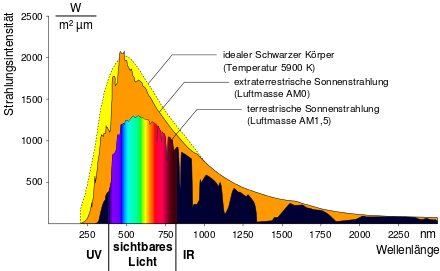
\includegraphics{sunspectrum}
			\caption{Intensitätsspektrum eines sonnenähnlichen Schwarzkörpers}
			\label{fig:Abb1}
		\end{figure}
		Hierzu benötigt man die Formeln für die spektrale Strahldichte und das Wien'sche Verschiebungsgesetz:
		\begin{align}
			L_{S,\lambda}(\lambda,T)&=\frac{\mathrm{c}_1}{\pi\lambda^{5}}\Big[\exp\Big(\frac{\mathrm{c}_2}{\lambda T}\Big)-1\Big]^{-1}\label{1}\\
			\lambda_{\mathrm{max}}T&=\SI{2.8978e-3}{\meter\kelvin}\label{2}
		\end{align}
		mit den Konstanten 
		\begin{align*}
			\mathrm{c}_1&=2\pi\planck\sol_0^2=\SI{3.7418e-16}{\watt\meter\squared}\\
			\mathrm{c}_2&=\planck\sol_0\boltz^{-1}=\SI{1.4388e-2}{\meter\kelvin}
		\end{align*}
		Die Sonnenoberfläche besitzt eine Temperatur von $T=\SI{5777}{\kelvin}$. Damit erreicht die Intensitätsverteilung ihr Maximum bei $\lambda_{\mathrm{max}}=\SI{5.016e-7}{\meter}$. Dies entspricht der Farbe Hellgrün. (Für Abbildung s. \hyperlink{Abb1}{hier})
		
	\item Wie hoch müsste die Temperatur eines schwarzen Körpers sein, damit das Intensitätsmaximum in der Mitte des sichbaren Bereichs liegt? Warum können solche Temperaturen nicht mit einem herkömmlichen Glühdraht erreicht werden?
		\subitem Nach dem Wien'schen Verschiebungsgesetz ergibt sich mit $\lambda_{\mathrm{avg}}=\SI{550}{\nano\meter}$:
		\begin{displaymath}
			T_{\mathrm{avg}}=\SI{5268}{\kelvin}
		\end{displaymath}
		Solche Temperaturen können mit herkömmlichen Glührähten aus Wolfram nicht erreicht werden, da Wolfram einen Schmelzpunkt von $T_{\mathrm{schmelz}}=\SI{3695}{\kelvin}$  aufweist.
	\item Wie kann die Temperatur eines Glühdrahtes relativ einfach (in guter Näherung) bestimmt werden, wenn der Verlauf des Spektrums der Strahlung bekannt ist? Wie kann diese bestimmt werden, wenn nur ein kleiner Ausschnitt des Verlaufs (z.B. nur der sichtbare Bereich) bekannt ist?
		\subitem Ist das gesamte Spektrum bekannt, so kann durch Ermittlung der Wellenlänge, bei der das Intensitätsmaximum auftritt, die Temperatur des Strahlers über das Wien'sche Verschiebungsgesetz recht einfach berechnen.
		Ist nur ein Teil des Spektrums bekannt, so kann aus dem Auftreten bestimmter Spektrallinien zumindest eine Mindesttemperatur extrapoliert werden, die nötig ist, um das Material des Glühdrahtes mit der entsprechenden Wellenlänge zum Leuchten zu bringen.
	\item Erklären Sie den Begriff der Farbtemperatur. Was sagt dieser Begriff über das Spektrum einer Glühlampe(Temperaturstrahler) und einer Energiesparlampe(Gasentladungslampe) aus?
		\subitem Unter Farbtemperatur versteht man die zu einer bestimmten Farbe gehörende Temperatur, die nötig ist, um einen schwarzen Körper unter festgelegter Helligkeit und  Beobachtungsbedingungen möglichst genau mit dieser Farbe zum Strahlen zu bringen. 
		
		Die Farbtemperatur von Energiesparlampen und anderen Gasentladungslampen ist im Normalfall bei ca. $\SI{4000}{\kelvin}-\SI{5000}{\kelvin}$ und damit höher, als bei Glühlampen (ca. $\SI{2600}{\kelvin}-\SI{3000}{\kelvin}$). Eine Ausnahme bilden hier lediglich Natriumdampflampen, deren Farbtemperatur etwa $\SI{2000}{\kelvin}$ beträgt. Damit ist im Allgemeinen eine höhere Temperatur nötig, um mit einem schwarzen Körper das Leuchten einer Energiesparlampe nachzuahmen, als das einer Glühbirne.
	\item Welcher proportionale Zusammenhang besteht zwischen spezifischer Ausstrahlung und Temperatur eines schwarzen Körpers? Welches Gesetz beschreibt diesen Zusammenhang?
		\subitem Wie oben bereits beschrieben, hängen die spezifische Ausstrahlung und Temperatur eines schwarzen Körpers über das Wien'sche Gesetz \eqref{2} zusammen.
	\item Wie kann mit Hilfe eines Spektrometers auf die chemischen Inhaltsstoffe von Gasentladungslampen geschlossen werden?
		\subitem Die Spektra von Gasentladungslampen haben meist sehr ausgeprägte Maxima, man spricht auch von Linienspektra. Vergleicht man die Wellenlängen dieser Peaks mit den Emissionsspektra von bekannten Stoffen, so lässt sich auf die chemische Zusammensetzung des jeweiligen Leuchtstoffs schließen.
\end{enumerate}
\section{Durchführung}
\subsection{Allgemeine Hinweise}
Zum Wechseln der Lampen (230 Volt!)
\begin{itemize}
	\item Lampe vor Wechseln ausschalten und abkühlen lassen
	\item Nicht die Kontakte in der Fassung berühren
\end{itemize}
Zum Umgang mit dem Lichtwellenleiter
\begin{itemize}
	\item Zu starke Krümmung vermeiden ($r\geq\SI{15}{\centi\meter}$)
	\item Unnötige Verspannungen des Knickschutzes vermeiden
	\item Berührungen mit dem Lichtwellenleitereingang vermeiden, diesen nach Versuchsende verschließen
	\item Abstand zwischen Lampe und Leiter min. $\SI{15}{\centi\meter}$
\end{itemize}
Zur Versuchsdurchführung
\begin{itemize}
	\item Auf möglichst wenig Umgebungslicht achten
	\item Dunkel- und Referenzspektrum aktuell halten
	\item Richtige Parameter beim Speichern angeben
	\item Diagramme mit allen relevanten Angaben beschriften
\end{itemize}
\subsection{Einführende Versuche}
\subsubsection{Einführung in SpectraWiz}
Öffnen Sie SpectraWiz und wechseln Sie ggf. in den Scope-Modus. Setze die Parameter folgendermaßen:
\begin{displaymath}
	\mathrm{\textsc{SCOPE -> ... Time: 100 ms, Avg:1, Sm:0, Sg:0, Tc:off, Xt:3, Ch:1}}
\end{displaymath}
Richten Sie den Lichtwellenleiter auf die Glühlampe aus und fixieren Sie ihn mithilfe des Stativmaterials. Speichern Sie bei abgeschalteter Lampe das Dunkelspektrum.
\begin{itemize}[label=$\blacktriangleright$]
	\item Wozu wird das Dunkelspektrum benötigt?
\end{itemize}
Justieren Sie den Lichtwellenleiter so, dass das Maximum des Graphen im obersten Viertel der Skala liegt.
\begin{itemize}[label=$\blacktriangleright$]
	\item Wie wirkt sich eine Änderung der Parameter "\textsc{Detector integration time}" und "\textsc{Number of scans to average}" auf die Anzeige aus?
\end{itemize}
Nehmen Sie das Spektrum der Glühlampe auf und speichern Sie es ab. 
\begin{itemize}[label=$\blacktriangleright$]
	\item Begründen Sie, warum die angezeigte Intensitätsverteilung nicht der tatsächlichen Verteilung des Glühlampenspektrums entsprechen kann.
\end{itemize}
\subsubsection{Aufnahme von Transmissionsspektren}
Nehmen Sie das Glülammpenspektrum als Referenzspektrum auf und wechseln Sie in den Transmissionsmodus
\begin{itemize}[label=$\blacktriangleright$]
	\item Wozu wird das Referenzsprektrum benötigt?
	\item Woran lässt ich im Transmissionsmodus erkennen, ob das Referenzspektrum und das Dunkelspektrum richtig eingestellt, bzw. ob die beiden noch aktuell sind?
	\item Warum ist im Wellenlängenbereich unterhalb von ca. $\SI{350}{\nano\meter}$ keine sinnvolle Transmissionsmessung möglich?
\end{itemize}
Halten Sie farbige Brillengläser in den Strahlengang.
\begin{itemize}[label=$\blacktriangleright$]
	\item Beschreiben Sie qualitativ Ihre Beobachtungen bzgl. der Farbe und des dazugehörigen Transmissionsspektrums.
\end{itemize}
Nehmen Sie die Transmissionsspektra zweier einzelner Gläser und dasd Spektrum der Kombination auf und speichern Sie sie ab. Stellen Sie die Spektra in QtiPlot in einem Diagramm dar und drucken Sie dieses aus.
\begin{itemize}[label=$\blacktriangleright$]
	\item Welcher mathematische Zusammenhang gilt für die einzelnen eben erwähnten Transmissionsgrade?
\end{itemize}
(\#) Ermitteln Sie in QtiPlot rechnerisch das Transmissionsspektrum der Filterkombination. Stellen Sie dieses zusammen mit den anderen Spektren in einem Diagramm dar.
\subsubsection{Aufnahme von Emissionsspektren}
Nehmen Sie im Scope-Modus das Spektrum einer Energiesparlampe auf und speichern Sie dieses ab.
\begin{itemize}[label=$\blacktriangleright$]
	\item Beschreiben Sie qualitativ die Unterschiede zum Spektrum einer Glühlampe.
\end{itemize}
Nehmen Sie die Spektren der LEDs (rot, grün, blau) auf.
\begin{itemize}[label=$\blacktriangleright$]
	\item Notieren Sie sich zu den einzelnen Farben der LEDs die Wellenlängenwerte der Maxima, welche Sie in SpectraWiz bestimmen können.
	\item Lässt sich durch diese Werte auf den jeweiligen Farbeindruck schließen? Begründen Sie Ihre Aussage.
\end{itemize}
\subsubsection{Bestimmung der Farbtemperatur einer Glühlampe}
Öffnen Sie in QtiPlot die Umrechnungstabelle und importieren Sie das Glühlampenspektrum. Führen Sie die für die Umrechnung erforderlichen Schritte aus und stellen Sie das angepasste Spektrum dar.
\begin{itemize}[label=$\blacktriangleright$]
	\item Warum müssen zur Bestimmung der Farbtemperatur die Messdaten umgerechnet werden?
	\item Begründen Sie qualitativ, wie und wie stark sich die angelegte Wechselspannung ($f=\SI{50}{\hertz}$) im Vergleich zu einer entsprechenden Gleichspannung auf die Farbtemperatur auswirkt.
\end{itemize}
Erstellen Sie mittels des Fit-Assistenten eine geeignete Kurve für den Wellenlängenbereich von ca. 1-2000nm. Drucken Sie das Diagramm, in dem die ermittelte Temperatur ersichtlich ist, aus.
\begin{itemize}[label=$\blacktriangleright$]
	\item Beschreiben Sie mit Hilfe des Graphen, warum eine Glühlampe als Beleuchtungsmedium nicht effizient ist.
	\item Bestimmen Sie mit Hilfe des Wien'schen Verschiebungsgesetzes die Lage des Maximums des angezeigten Schwarzkörperspektrums.
\end{itemize}
\subsection{Erzeugung verschiedener Farbtemperaturen mit einem Glühlämpchen}
Nehmen Sie drei verschiedene Spektra durch Änderung der Spannung (max. 10 Volt!) zu den subjektiv empfundenen Intensitäten "schwach", "mittel" und "stark" auf.

Ermitteln Sie in QtiPlot die Farbtemperaturen und speichern Sie die Diagramme ab.
\begin{itemize}[label=$\blacktriangleright$]
	\item Begründen Sie qualitativ, wie und warum sich die angelegte elektrische Spannung auf das aufgenommene Spektrum auswirkt.
\end{itemize}
\subsection{Auswertung des Sonnenspektrums}
\subsubsection{Aufnahme des Sonnenspektrums}
Richten Sie den Lichtwellenleiter so aus, dass Sie das Sonnenspektrum aufnehmen können (Aufnahme des Streulichts genügt). Speichern Sie bei aktuell gehaltenem Dunkelspektrum die Intensitätsverteilung ab.
\subsubsection{Bestimmung der Oberflächentemperatur der Sonne}
Rechnen Sie die Messdaten in QtiPlot um und stellen Sie sie graphisch dar. Erstellen Sie eine Fit-Kurve* und drucken Sie das Diagramm mit Angabe der ermittelten Oberflächentemperatur aus.

*Für den Fall, dass keine geeignete Kurve ermittelt werden kann, stellen Sie den Verlauf eines Schwarzkörperspektrums für $T=\SI{6000}{\kelvin}$ dar.
\begin{itemize}[label=$\blacktriangleright$]
	\item Begründen Sie kurz einige bei dieser Auswertung vorliegende Fehlerquellen.
\end{itemize}
\subsubsection{Bestimmung der wichtigsten Fraunhofer'schen Linien}
Stellen Sie das Sonnenspektrum in einem neuen Diagramm dar. Drucken Sie den Graphen aus. Bestimmen Sie mit Hilfe des "Datenlesers" die Wellenlängen der "Einbrüche" im Spektrum, welche den jeweiligen Fraunhofer'schen Linien entsprechen (vgl. Tabelle).		
\begin{enumerate}[label=$\blacktriangleright$]
	\item Kennzeichnen Sie die Lage diser Linien im Diagramm.
	\item Notieren Sie die gemessenen Wellenlängenwerte und bestimmen Sie die Differenz zu den Tabellenwerten.
	\item Wie lässt sich diese Differenz erklären?
\end{enumerate}
\begin{table}
	\caption{Wichtige Fraunhofer'sche Linien} \label{tab: flines}
	\centering
	\begin{tabular}{>{\bfseries}lll}
		\toprule[2pt]	Symbol&$\lambda$[nm]&Element\\
		\midrule[2pt]	A&$760.8$&\ce{O}\\
		\midrule		B&$686.7$&\ce{O}\\
		\midrule		C&$656.3$&\ce{H}\\
		\midrule		D\textsubscript{1}&$589.6$&\ce{Na}\\
		\midrule		D\textsubscript{2}&$589.0$&\ce{Na}\\
		\midrule		E&$527.0$&\ce{Fe}\\
		\midrule		F&$486.1$&\ce{H}\\
		\midrule		G&$430.8$&\ce{Fe}\\
		\midrule		H&$396.8$&\ce{Ca}\\
		\midrule		K&$393.4$&\ce{Ca}\\
		\bottomrule[2pt]
	\end{tabular}
\end{table}
\subsection{Bestimmung chemischer Elemente}
Stellen Sie das Spektrum einer Glimmlampe im Scope-Modus dar. Dieses erhalten Sie durch Aufnahme der Schalterbeleuchtung einer Steckdosenleiste. Justieren Sie hierzu den Lichtwellenleiter senkrecht über dem Schalter in wenigen Zentimetern Abstand.
\begin{enumerate}[label=$\blacktriangleright$]
	\item Erläutern Sie qualitativ, ob und wie der transparente gefärbte Kunststoff des Schalters die Aufnahme des Spektrums beeinflusst.
	\item Warum ist für diesen Versuchsteil keine Umrechnung der Daten in QtiPlot notwendig?
\end{enumerate}
Werten Sie das abzuspeichernde Spektrum in QtiPlot aus. Bestimmen Sie mittels ausliegender Messdaten bekannter Stoffe das für die Strahlung verantwortliche Element in der Lampe.

Importieren Sie zusätzlich die Messdaten des passenden Vergleichsspektrums und stellen Sie dieses im gleichen Diagramm dar.
\begin{enumerate}[label=$\blacktriangleright$]
	\item Welchen Vorteil hat dieses Verfahren gegenüber der Auswertung mit Hilfe von Tabellenwerten?
\end{enumerate}
Beschriften Sie markante Peaks mit zugehörigen Wellenlängen und drucken Sie das Diagramm aus.

(\#)Belegen Sie graphisch, dass in einer Energiesparlampe Anteile von Quecksilber vorhanden sind. Drucken Sie anschließend Ihre Ergebnisse mit geeigneter Beschriftung aus.
\subsection{Additive Farbmischung}
Betrachten Sie im Scope-Modus das Spektrum der farbwechselnden LED-Lampe und beantworten Sie folgende Fragen:
\begin{enumerate}[label=$\blacktriangleright$]
	\item Wie viele verschiedenfarbige LEDs werden in dieser Lampe eingesetzt?
	\item Welche (Peak-)Wellenlängen und Farben haben diese LEDs?
	\item Nennen Sie zusätzlich ein Beispiel, an dem ersichtlich wird, warum aufgrund eines Farbeindrucks nicht auf die zugrundeliegenden Wellenlängen geschlossen werden kann.
\end{enumerate}
Veranschaulichen Sie sich die additive Farbmischung mittels LEDs, deren Helligkeit einzeln verändert werden kann. Versuchen Sie, Mischfarben zu erzeugen. Verwenden Sie die Lampe als Streumedium. Richten Sie die LEDs auf eine weiße Fläche und erzeugen Sie Schatten in verschiedenen Farben.
\begin{enumerate}[label=$\blacktriangleright$]
	\item Erklären Sie das Zustandekommen dieser bunten Schatten.
\end{enumerate}